\documentclass{article}
\usepackage[utf8]{inputenc}
\usepackage{indentfirst}
\usepackage{titling}
\usepackage{geometry}
\usepackage{graphicx}
\graphicspath{ {./Images/} }
\usepackage[shortlabels]{enumitem}
\usepackage{fancyhdr}
\usepackage{ulem}
\usepackage[dvipsnames]{xcolor}
\usepackage{amssymb}
\usepackage{listings}
\usepackage{color}

\definecolor{dkgreen}{rgb}{0,0.6,0}
\definecolor{gray}{rgb}{0.5,0.5,0.5}
\definecolor{mauve}{rgb}{0.58,0,0.82}

\lstset{frame=tb,
  language=Java,
  aboveskip=3mm,
  belowskip=3mm,
  showstringspaces=false,
  columns=flexible,
  basicstyle={\small\ttfamily},
  numbers=none,
  numberstyle=\tiny\color{gray},
  keywordstyle=\color{blue},
  commentstyle=\color{dkgreen},
  stringstyle=\color{mauve},
  breaklines=true,
  breakatwhitespace=true,
  tabsize=3
}

\def\ojoin{\setbox0=\hbox{$\bowtie$}%
  \rule[-.02ex]{.25em}{.4pt}\llap{\rule[\ht0]{.25em}{.4pt}}}
\def\leftouterjoin{\mathbin{\ojoin\mkern-5.8mu\bowtie}}
\def\rightouterjoin{\mathbin{\bowtie\mkern-5.8mu\ojoin}}
\def\fullouterjoin{\mathbin{\ojoin\mkern-5.8mu\bowtie\mkern-5.8mu\ojoin}}

\renewcommand\maketitlehooka{\null\mbox{}\vfill} %para centralizar verticalmente
\renewcommand\maketitlehookd{\vfill\null}
\pagestyle{fancy}
\fancyhf{}
\rfoot{\thepage}
\lfoot{ 
\includegraphics[scale=0.01]{UA.jpg} José Mendes 107188 LEI}
\geometry{
  a4paper,
  headheight=4cm,
  top=5.5cm,
  bottom=4.5cm,
  footskip=4cm
}


\title{Tecnologias e Programação Web}
\author{José Mendes 107188}
\date{2023/2024}

\begin{document}


\begin{titlepage}
    \maketitle
    \begin{center}
        
\includegraphics[scale=0.4]{UA.png}
    \end{center}
    \thispagestyle{empty} %remove o count da pagina
\end{titlepage}

\pagebreak
%depois por um index aqui

\section{Arquiteturas de Aplicações Web}

\subsection{Independência dos Dados nas Bases de Dados}

\subsubsection{Arquitetura da Base de Dados e Views}

\begin{center}
    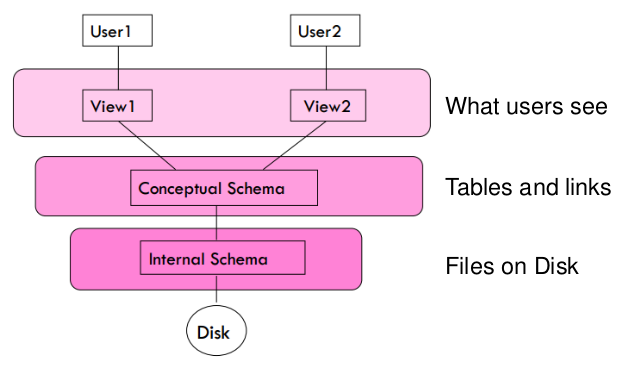
\includegraphics[scale=0.4]{1}
\end{center}

\subsubsection{Independência Lógica e Física}

\begin{center}
    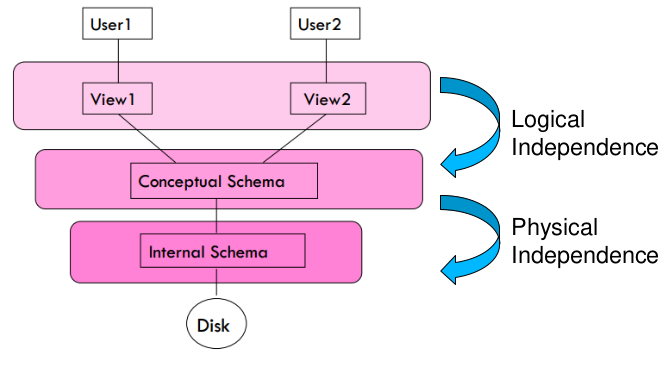
\includegraphics[scale=0.4]{2}
\end{center}

\begin{flushleft}
  Cada nível é independente dos níveis a baixo.
\end{flushleft}

\pagebreak

\subsubsection{Independência dos Dados}

\begin{flushleft}
  \textbf{Independência Física:} Capacidade de alterar o schema interno sem alterar
  o schema conceptual.
  \begin{itemize}
    \item Espaço de armazenamento pode mudar;
    \item O tipo de alguns dados pode mudar por razões de eficiência/otimização;
  \end{itemize}

  \textbf{Independência Lógica:} Capacidade de alterar o schema conceptual sem alterar
  as Views ou os programas de aplicação.
  \begin{itemize}
    \item Pode adicionar novos campos, novas tabelas sem alterar as Views;
    \item Pode alterar a estrutura das tabelas sem alterar as Views;
  \end{itemize}

  \vspace{5mm}

  \textbf{Nota:} Manter a \textbf{View} (aquilo que o user vê) \uline{independente} do \textbf{Modelo} (domain knowledge).
\end{flushleft}

\subsection{Arquiteturas N-Tier}

\subsubsection{Significado de "Tiers"}

\begin{flushleft}
  Arquiteturas N-Tier têm as mesmas camadas:
  \begin{itemize}
    \item \textbf{Presentation Tier:} Camada de apresentação;
    \item \textbf{Business/Logic Tier:} Camada de lógica/de negócio;
    \item \textbf{Data Tier:} Camada de dados;
  \end{itemize}

  Arquiteturas N-Tier tentam separar as camadas em diferentes tiers.
  \begin{itemize}
    \item \textbf{Camada}: Separação lógica;
    \item \textbf{Tier}: Separação física;
  \end{itemize}
\end{flushleft}

\subsubsection{Arquitetura 1-Tier}

\begin{center}
  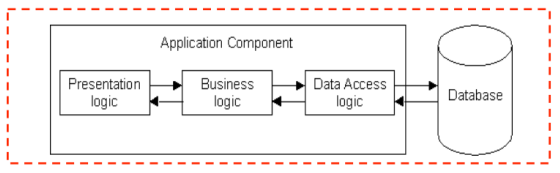
\includegraphics[scale=0.4]{3}
\end{center}

\begin{flushleft}
  As 3 camadas estão no mesmo computador (máquina). Isto é, todo o código e processamento
  está numa única máquina.

  As camadas de apresentação, lógica e de dados estão firmemente conectados.
  \begin{itemize}
    \item \textbf{Escalabilidade:} Um único processador implica que é díficil de
    aumentar o volume de processamento;
    \item \textbf{Portabilidade:} Mudar para outro computador pode implicar
    reescrever tudo;
    \item \textbf{Manutenção:} Mudar uma camada requer mudar outras camadas;
  \end{itemize}
\end{flushleft}


\subsubsection{Arquitetura 2-Tier}

\begin{center}
  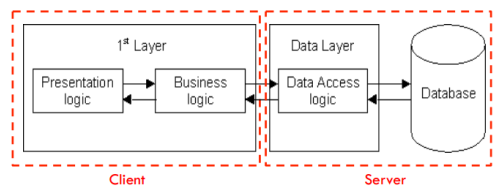
\includegraphics[scale=0.4]{4}
\end{center}

\begin{flushleft}
  A base de dados corre no servidor, separado do cliente, sendo fácil de
  mudar para uma base de dados diferente.

  As camadas de apresentação e lógica ainda estão firmemente conectados.
  \begin{itemize}
    \item Carga pesada no servidor;
    \item Potencial congestionamento da rede;
    \item Apresentação ainda está firmemente conectada à lógica de negócio;
  \end{itemize}
\end{flushleft}

\subsubsection{Arquitetura 3-Tier}

\begin{center}
  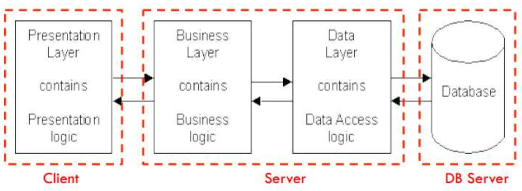
\includegraphics[scale=0.4]{5}
\end{center}

\begin{flushleft}
  Cada camada pode, potencialmente, correr numa máquina diferente.
  As camadas de apresentação, lógica e de dados estão disconectadas. 
\end{flushleft}

\begin{flushleft}
  \textbf{Típica Arquitetura 3-Tier}
\end{flushleft}

\vspace{5mm}

\begin{center}
  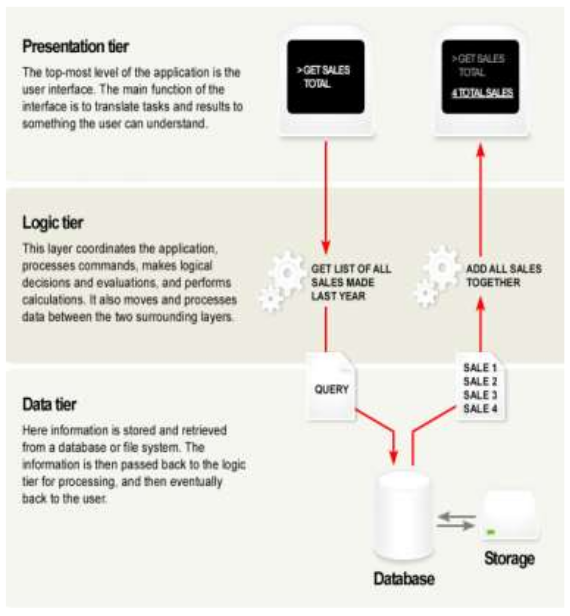
\includegraphics[scale=0.3]{6}
\end{center}


\pagebreak

\begin{flushleft}
  \textbf{Princípios de Arquitetura:}
  \begin{itemize}
    \item Arquitetura \textbf{Cliente-Servidor};
    \item Cada camada (Apresentação, Lógica, Dados) deve ser independente e não deve
    expôr dependências relacionadas com a implementação;
    \item Camadas disconectadas não devem comunicar;
    \item Alterações numa plataforma afetam apenas a camada que corre que essa plataforma;
  \end{itemize}

  \textbf{Camada de Apresentação:}
  \begin{itemize}
    \item Fornece a interface do utilizador;
    \item Lida com a interação com o utilizador;
    \item Por vezes chamada de GUI, client view ou \textbf{front-end};
    \item Não deve conter lógica de negócio ou código de acesso aos dados;
  \end{itemize}

  \textbf{Camada de Lógica:}
  \begin{itemize}
    \item O conjunto de regras para processar a informação;
    \item Pode acomodar vários utilizadores;
    \item Por vezes chamada de \textbf{middleware} ou back-end;
    \item Não deve conter apresentação ou código de acesso aos dados;
  \end{itemize}

  \textbf{Camada de Dados:}
  \begin{itemize}
    \item A camada de armazenamento físico, para persistir os dados;
    \item Gere o acesso à base de dados ou sistema de ficheiros;
    \item Por vezes chamada de \textbf{back-end};
    \item Não deve conter apresentação ou código da lógica de negócio;
  \end{itemize}
\end{flushleft}

\subsubsection{Arquitetura 3-Tier para Aplicações Web}

\begin{flushleft}
  \textbf{Camada de Apresentação:} Conteúdo estático ou dinâmico, renderizado pelo browser (\textbf{front-end});
  
  \textbf{Camada de Lógica:} Processamento de conteúdo dinâmico, geração de servidores de aplicação
  (e.g. Java EE, ASP.NET, Python Django Framework) (\textbf{middleware});
  
  \textbf{Camada de Dados:} Base de dados, composta por ambos, conjunto dos dados e o sistema de gestão de base de dados
  ou software RDBMS que gere e fornece acesso aos dados (\textbf{back-end});
\end{flushleft}

\pagebreak

\subsubsection{Arquitetura 3-Tier - Vantagens}

\begin{flushleft}
  \textbf{Independência das camadas}
  \begin{itemize}
    \item Mais fácil de manter;
    \item Componentes são reutilizáveis;
    \item Desenvolvimento mais rápido (divisão do trabalho, 
    Web Designer faz a apresentação, Engenheiros de Software fazem a lógica
    e administradoes de base de dados fazem o modelo de dados);
  \end{itemize}
\end{flushleft}

\subsection{Padrões de Desenho}

\subsubsection{Padrões de Desenho e Decisões}

\begin{flushleft}
  \begin{itemize}
    \item Contrução e teste;
    \begin{itemize}
      \item como contruímos uma aplicação web?
      \item que tecnologias devemos escolher?
    \end{itemize}

    \item Reutilizar;
    \begin{itemize}
      \item podemos usar componentes normais?
    \end{itemize}

    \item Escalabilidade;
    \begin{itemize}
      \item como vai a nossa aplicação web lidar com um elevado número de pedidos?
    \end{itemize}

    \item Segurança;
    \begin{itemize}
      \item como proteger contra um attack, vírus, acesso malicioso dos dados, denial of service?
    \end{itemize}


    \item Diferentes views de dados;
    \begin{itemize}
      \item tipos de users, contas individuais, proteção de dados
    \end{itemize}
  \end{itemize}

  \vspace{5mm}
  \textbf{Nota:} Precisamos de uma solução geral e reutilizável: \textbf{Padrões de Desenho}
\end{flushleft}

\subsubsection{O que é um Padrão de Desenho?}

\begin{flushleft}
  Uma solução geral e reutilizável para um problema recorrente no desenho de software.
  É um template para como resolver um problema que tenha sido usado em várias situções diferentes.

  \textbf{NÂO} é um design completo, o padrão precisa de ser adaptado à aplicação,
  não podemos simplesmente traduzir o padrão para código.
\end{flushleft}

\pagebreak

\subsubsection{Origem do Padrão de Desenho}

\begin{flushleft}
  \begin{itemize}
  \item Arquitetura conceptual por Christopher Alexander (1977/1979).
  \item Adaptado para programação OO por Kent Beck e Ward Cunningham (1987).
  \item Ganhou popularidade em CS com o livro "Design Patterns: Elements of Re-usable Object-Oriented Software" (1994),
  por Erich Gamma, Richard Helm, Ralph Johnson e John Vlissides (Gang of Four).
  \item Agora bastante utilizado em Engenheiria de Software.
  \end{itemize}
\end{flushleft}

\subsection{O Padrão de Desenho MVC}

\subsubsection{O Problema do Desenho}

\begin{flushleft}
  \begin{itemize}
    \item Preciso mudar o look-and-feel sem mudar o core/logic;
    \item Preciso de apresentar os mesmos dados de diferentes formas (e.g. computadores bons, web, dispositivos móveis);
    \item Preciso de interagir/acessar os dados de diferentes formas (e.g. ecrã tátil nos dispositivos móveis, teclado no computador);
    \item Preciso de manter várias views para a mesma informação (e.g lista, thumbnails, detalhes, \dots);
  \end{itemize}
\end{flushleft}

\subsubsection{A Solução do Desenho}

\begin{flushleft}
  \begin{itemize}
    \item Separar a funcionalidade chave da apresentação e lógica que usa esta funcionalidade;
    \item Permitir múltiplas views para partilhar o mesmo modelo de dados;
    \item Tornar o suporte de vários clientes mais fácil de implementar, testar e manter;
  \end{itemize}
\end{flushleft}

\subsubsection{O Padrão Model-View-Controller}

\vspace{3mm}

\begin{center}
  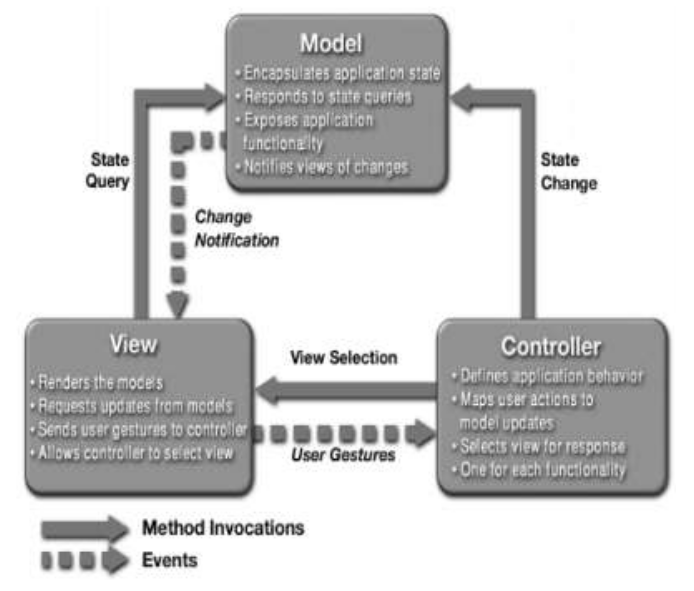
\includegraphics[scale=0.3]{7}
\end{center}

\pagebreak

\begin{flushleft}
  Padrão de Desenho para sistemas gráficos que \textbf{promove a separação entre o modelo e a view}.
  Com este padrão, a lógica necessária para manutenção dos dados (base de dados, ficheiro de texto),
  \textbf{é separada} de como os dados são apresentados (gráfico, numerico) e como
  os dados são manipulados (GUI, linha de comandos, touch).
\end{flushleft}

\begin{flushleft}
  \textbf{Model}
  \begin{itemize}
    \item Gere o comportamento e os dados do domínio da aplicação;
    \item Responde a pedidos por informação sobre o estado (normalmente da view),
    segue instruções para alterar o estado (normalmente do controller);
  \end{itemize}

  \textbf{View}
  \begin{itemize}
    \item Renderiza o modelo para uma forma apropriada para a interação,
    tipicamente uma interface do utilizador (várias views podem existir para o mesmo modelo
    com diferentes intenções);
  \end{itemize}

  \textbf{Controller}
  \begin{itemize}
    \item Recebe os inputs e inicia uma resposta realizando chamadas em objetos do modelo;
    \item Aceita input do utilizador e intrui o modelo e a view para realizar ações baseadas no input;
  \end{itemize}
\end{flushleft}


\subsubsection{O Padrão MVC na prática}

\begin{flushleft}
  \textbf{Model}
  \begin{itemize}
    \item Contém conhecimento específico do domínio;
    \item Regista o estado da aplicação (e.g quais items estão no carrinho de compras);
    \item Normalmente conectado com a base de dados;
    \item Independente da view (um model pode ter várias views);
  \end{itemize}

  \textbf{View}
  \begin{itemize}
    \item Apresenta dados ao utilizador;
    \item Permite interação com o utilizador;
    \item Não faz processamento;
  \end{itemize}
    
  \textbf{Controller}
  \begin{itemize}
    \item Define como a interface do utilizador reage a inputs (eventos);
    \item Recebe mensagens da view (de onde os eventos vêm);
    \item Envia mensagens ao modelo (diz quais dados mostrar)
  \end{itemize}
\end{flushleft}

\pagebreak

\subsubsection{O MVC para Aplicações Web}

\begin{flushleft}
  \textbf{Model}
  \begin{itemize}
    \item Tabelas da base de dados (dados persistentes);
    \item Informações sobre a sessão (dados atuais do sistema de dados)
    \item Regras sobre transações;
  \end{itemize}

  \textbf{View}
  \begin{itemize}
    \item (X)HTML;
    \item CSS style sheets;
    \item Templates server-side;
  \end{itemize}

  \textbf{Controller}
  \begin{itemize}
    \item Scripts client-side;
    \item Processamento de pedidos HTTP;
    \item Lógica de negócio/preprocessamento;
  \end{itemize}
\end{flushleft}

\subsubsection{MVC - Vantagens}

\begin{flushleft}
  \textbf{Clareza de Design}
  \begin{itemize}
    \item métodos do modelo dão uma API para os dados e o estado;
    \item o design da view e do controller são fáceis; 
  \end{itemize}

  \textbf{Modularidade eficiente}
  \begin{itemize}
    \item qualquer componente pode ser facilmente substituído;
  \end{itemize}

  \textbf{Várias views}
  \begin{itemize}
    \item Várias views podem ser criadas conforme apropriado;
    \item Cada uma usa a mesma API para o modelo;
  \end{itemize}

  \textbf{Mais fácil de contruir e manter}
  \begin{itemize}
    \item Views simples (baseado em texto) durante o desenvolvimento (contrução);
    \item Mais views e controllers podem ser adicionados mais tarde;
    \item Fácil de contruir interfaces estáveis;
  \end{itemize}

  \textbf{Distribuível}
  \begin{itemize}
    \item Ajuste natural para ambientes distribuídos;
  \end{itemize}
\end{flushleft}

\pagebreak

\subsubsection{3-Tier Architecture vs Padrão MVC}

\begin{flushleft}
  \begin{itemize}
    \item Comunicação
    \begin{itemize}
      \item \textbf{3-Tier:} A camada de apresentação nunca comunica diretamente
      com a camada de dados, apenas através da camada de lógica (topologia linear);
      \item \textbf{MVC:} Todas as camadas comunicam diretamente (topologia triangular);
    \end{itemize}

    \item Usabilidade
    \begin{itemize}
      \item \textbf{3-Tier:} É usada em aplicações web onde os tiers cliente, middleware
      e os dados corram em plataformas fisicamente separadas;
      \item \textbf{MVC:} Historicamente usada em aplicações que correm numa única estação de trabalho gráfica;
      \begin{itemize}
        \item No contexto de aplicações web, contudo, os componentes lógicos podem ser
        desacoplados para cumprir com uma verdadeira arquitetura 3-Tier;
      \end{itemize}
    \end{itemize}
  \end{itemize}
\end{flushleft}

\section{Introdução à Plataforma Django}

\subsection{Introdução}

\begin{flushleft}
  \textbf{Django} é uma plataforma gratuita e open-sourc, escrita em Python,
  para o desenvolvimento de aplicações web.
  Tem o nome do famoso guitarrista de jazz Django Reinhardt.
  É mantida pela Django Software Foundation (DSF), uma organização independente.
  Fomenta o desenvolvimento rápido, limpo e pragmático.
  Criada em 2003, lançada open-source em 2005.
\end{flushleft}

\subsection{Características}

\begin{flushleft}
  \begin{itemize}
    \item Segue, parcialmente, o padrão MVC;
    \item Possuuie um ORM (Object-Relational Mapper) para processar dados;
    \item Focada na automatização, aderinco ao princípio DRY (Don't Repeat Yourself);
    \item Usa um sistema de templates;
    \item Sistema de personalização Admin, para facilitar o CRUD;
    \item Desenho elegante de routing de URLs;
    \item Possui um light web server embotido (para testes);
    \item Possibilita a utilização de moddleware personalizado;
    \item Possui facilidades para: autenticação, internacionalização, caching;
  \end{itemize}
\end{flushleft}

\pagebreak

\subsection{Arquitetura}

\begin{center}
  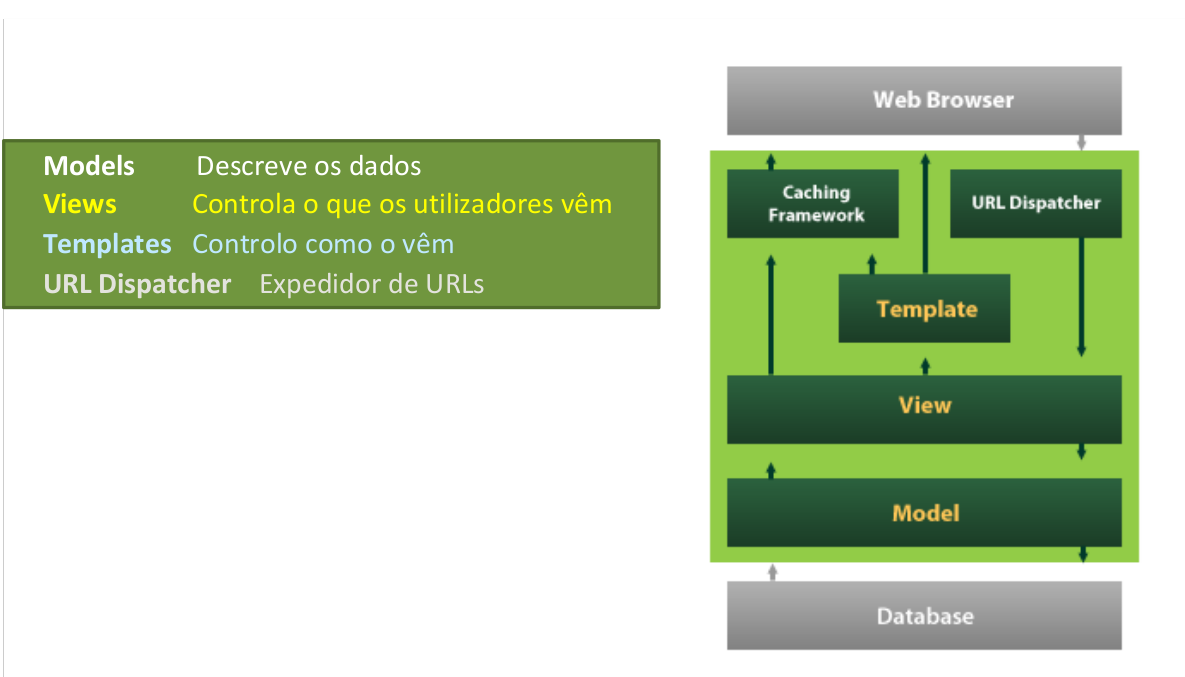
\includegraphics[scale=0.3]{8}
\end{center}

\subsection{Estrutura de um Projeto Django}

\begin{center}
  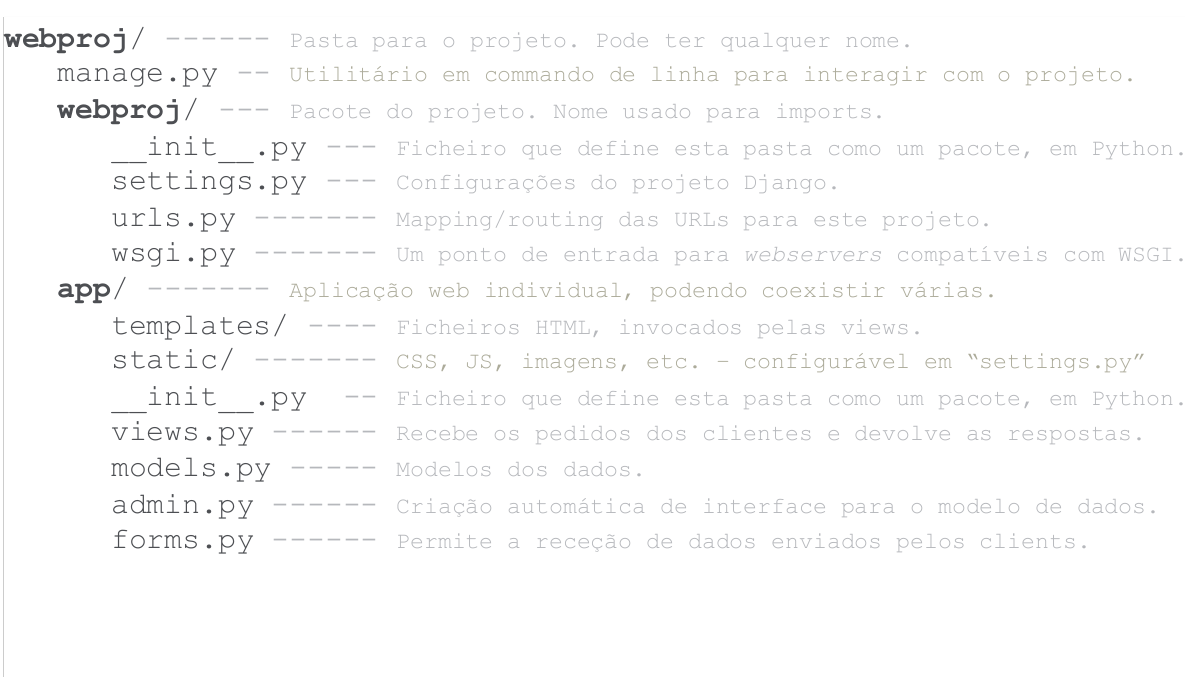
\includegraphics[scale=0.3]{9}
\end{center}

\pagebreak

\subsection{Settings}

\begin{flushleft}
  Possui um ficheiro de configuração, \textbf{settings.py},
  do projeto Django, sobrepõe as configurações padrão
  (ficheiro <python>/lib/sitepackages/django/conf/global\_settings.py).

  \vspace{2mm}
  Possui alguns atributos como: \textbf{DEBUG} (True/False),
  \textbf{DATABASES ENGINES} (sqlite3, mysql, postgresql, oracle),
  \textbf{ROOT\_URLCONF} (nome do ficheiro de routing de URLs),
  \textbf{MEDIA\_ROOT} (para ficheiros enviados pelo utilizador),
  \textbf{MEDIA\_URL} (para ficheiros multimédia),
  \textbf{STATIC\_ROOT} (pasta para ficheiros estáticos, CSS, JS),
  \textbf{STATIC\_URL} (pasta de ficheiros estáticos),
  \textbf{TEMPLATE\_DIRS} (pasta de templates)
\end{flushleft}

\subsection{Criação de um Projeto Django}

\begin{flushleft}
  Nesta cadeira vamos usar o PyCharm, pelo que para criar um projeto Django
  basta selecionar a opção \textbf{Django} e chamar a pasta dos templates de
  \textbf{app/templates} e a pasta da aplicação de \textbf{app}.
  
  Para correr basta clicar em Run e aceder ao link \textbf{http://127.0.0.1:8000}.

  Ou podemos usar o comando \textbf{python manage.py runserver}.
\end{flushleft}

\subsubsection{Views}

\begin{flushleft}
  No ficheiro "app/views.py"  podemos inserir views:
\end{flushleft}

\begin{center}
  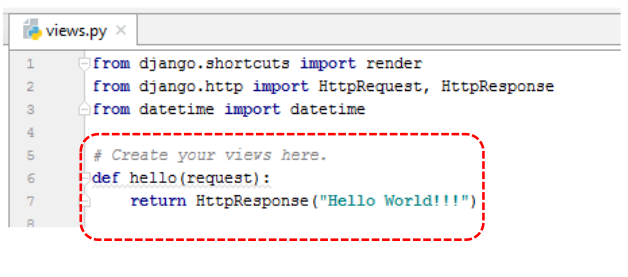
\includegraphics[scale=0.3]{10}
\end{center}

\begin{flushleft}
  Para criar uma nova, basta criar uma nova view function.
\end{flushleft}

\subsubsection{Configuração da URL}

\begin{flushleft}
  No ficheiro "nome\_do\_projeto/urls.py" podemos configurar as URLs:
\end{flushleft}

\begin{center}
  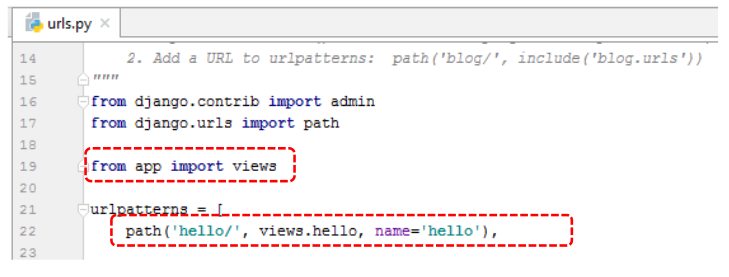
\includegraphics[scale=0.3]{11}
\end{center}

\begin{flushleft}
  Para criar uma nova, basta inserir mais uma route para a view.
\end{flushleft}

\subsubsection{Templates}

\begin{flushleft}
  Podemos usar variáveis usando \{\{ var\_name \}\} e template tags (como if)
  usando \{\% if \dots \%\}.
\end{flushleft}

\pagebreak

\subsubsection{Ficheiros estáticos}

\begin{flushleft}
  São ficheiros que se pretende simplesmente referenciar e servir ao cliente,
  sem qualquer processamento prévio.

  O seu acesso é público, pois o cliente apenas necessita do URL para os mesmos.

  Exemplos:
  \begin{itemize}
    \item Imagens (jpg, png, gif, \dots);
    \item Style Sheets (CSS);
    \item Scripts (JavaScript);
    \item \dots
  \end{itemize}
\end{flushleft}

\subsubsection*{Localização}

\begin{flushleft}
Os ficheiros denominados por static files
residem em pastas pré-determinadas, dentro
ou fora da “app” (normalmente uma pasta denominada de "static").
\end{flushleft}

\subsubsection*{Configuração}

\begin{flushleft}
  No ficheiro "settings.py" podemos configurar os ficheiros estáticos:
  \begin{enumerate}
    \item o módulo 'django.contrib.staticfiles' deve aparecer
    nas aplicações instaladas “INSTALLED\_APPS”
    \item o atributo STATIC\_URL deve ser definido (ex: '/static/')
    \item a pasta dos static files deve estar definida no atributo STATIC\_ROOT
    (ex: os.path.join(BASE\_DIR, 'app/static'))
  \end{enumerate}
\end{flushleft}

\subsubsection*{Uso}

\begin{flushleft}
  Para usar basta usar a tag \{\% load static \%\} e depois
  referenciar o ficheiro.
\end{flushleft}

\subsection{Modelos - Camada de Base de Dados Django}

\subsubsection{Modelo}

\begin{flushleft}
  \begin{itemize}
    \item MTV - Model-Template-View;
    \item Modelo
    \begin{itemize}
      \item Consiste na camada de acesso aos dados - "Data Access Layer";
      \item Esta camada permite definir, em relação aos dados:
      o \textbf{Acesso}, a \textbf{Validação}, o \textbf{Comportamento} e as \textbf{Relações} entre os dados;
    \end{itemize}
  \end{itemize}
\end{flushleft}

\pagebreak

\subsubsection{Configuração da Base de Dados}

\begin{flushleft}
  No ficheiro "settings.py" podemos configurar a base de dados,
  basta procurar pela variável \textbf{DATABASES} e definir os parâmetros
  \textbf{ENGINE}, \textbf{NAME}, \textbf{USER}, \textbf{PASSWORD},
  \textbf{HOST}, \textbf{PORT}.

  Por defeito, o Django usa o SQLite3.
\end{flushleft}

\subsubsection{Criação de um modelo}

\begin{flushleft}
  A criação de modelos vai acontecer no ficheiro "app/models.py".
  Para criar um modelo basta criar uma classe que herde de \textbf{models.Model}.
  Os atributos da classe são os campos da tabela.

  \vspace{2mm}

  Para cada atributo das classes é instanciado um
  objeto tipo “Field” e/ou subtipo, como: \textbf{CharField},
  \textbf{DataField}, etc.

  Alguns atributos, representam a criação de relações
  entre as classes, tendo como efeito a criação de
  colunas com chaves estrangeiras (\textbf{1:1}, \textbf{1:M}, \textbf{M:1}) ou
  de tabelas de associação (\textbf{M:N})

  \vspace{3mm}

  \textbf{Relações entre classes:}

  \begin{itemize}
    \item \textbf{1:M e M:1}
    \begin{itemize}
      \item Conseguida com o atributo \textbf{models.ForeignKey};
      \item \uline{Exemplo}: Publisher (1) : (M) Book ou Book (M) : (1) Publisher
      O atributo é colocado na classe que representa o lado “M” da relação, neste caso a classe Book;
    \end{itemize}

    \item \textbf{1:1} (único)
    \begin{itemize}
      \item Conseguida com o atributo \textbf{models.OneToOneField};
      \item \uline{Exemplo}: Book (1) : (1) Place
      O atributo "deve" ser colocado na classe que mais necessita da outra, neste caso a classe Book;
    \end{itemize}

    \item \textbf{M:N}
    \begin{itemize}
      \item Conseguida com o atributo \textbf{models.ManyToManyField};
      \item \uline{Exemplo}: Book (M) : (N) Author
      O atributo “deve” ser colocado na classe que mais “necessita” da
outra, como na relação de 1:1 
    \end{itemize}
  \end{itemize}

  A classe base “Model”, donde são derivadas todas as
  classes do modelo, possui todos os mecanismos
  necessários para interagir com a base de dados.

  Cada classe derivada é implementada na BD na
  forma de uma tabela e os seus atributos são
  implementados na forma de colunas (campos) da
  tabela.

  Com vista à ativação do modelo, a aplicação web, “app”, deve
  ser incluída na variável \textbf{INSTALLE\_APPS} do ficheiro
  “settings.py”. Caso a aplicação já esteja a ser incluída, de
  forma indireta, não é necessário.
\end{flushleft}

\pagebreak

\subsubsection{Comandos na criação de um modelo}

\begin{flushleft}
  \textbf{python manage.py check} - valida o modelo (sintaxe e lógica)

  \textbf{python manage.py makemigrations} - produz código de migração (na
  pasta \uline{app/migrations} devemos apagar tudo menos o ficheiro \uline{\_\_init\_\_.py})
  
  \textbf{python manage.py sqlmigrate app 0001} - mostra o SQL gerado pela migração

  \textbf{python manage.py migrate} - produz as tabelas na BD
\end{flushleft}

\subsubsection{Gestão dos Dados}

\begin{flushleft}
  A plataforma Django possui um mecanismo
  que possibilita uma gestão muito facilitada de
  todos os dados pertencentes ao modelo de
  dados: o Django Admin Site

  A URL = \textbf{http://localhost:{port}/admin} dá acesso
  à área administrativa a qual permite, por
  defeito, gerir os utilizadores do site

  Nesta érea, também é possível aceder e gerir
  os dados definidos no modelo

  Para tal, é necessário no ficheiro "urls.py" da
  aplicação adicionar:
  \begin{itemize}
    \item o import "\textbf{from django.contrib import admin}"
    \item a linha "\textbf{path('admin/', admin.site.urls)}"
  \end{itemize}

  Também é necessário registar as classes que se pretende gerir:
  \begin{itemize}
    \item o mesmo import que em cima
    \item importar as classes que se pretende gerir de "\textbf{app.models}"
    \item adicioná-los: "\textbf{admin.site.register(Class)}"
  \end{itemize}

  Por fim é necessário criar a conta de administração, com o comando:
  \textbf{python manage.py createsuperuser}

  \vspace{2mm}

  \textbf{Programando:}
  \begin{itemize}
    \item Inserir um objeto:
    \begin{lstlisting}
      a = Author(name="Jose", email="mendes.j@ua.pt")
      a.save()
    \end{lstlisting}

    \item Modificar um objeto:
    \begin{lstlisting}
      a.email = "ze.mendes@ua.pt"
      a.save()
    \end{lstlisting}

    \item Selecionar todos os objetos:
    \begin{lstlisting}
      Author.objects.all()
    \end{lstlisting}

    \pagebreak

    \item Filtrar objetos (por nome):
    \begin{lstlisting}
      Autor.objects.filter(name="Jose")
    \end{lstlisting}

    \item Filtrar por nome e por email:
    \begin{lstlisting}
      Autor.objects.filter(name="Jose", email="mendes.j@ua.pt")
    \end{lstlisting}

    \item Filtrar por nome parecido:
    \begin{lstlisting}
      Autor.objects.filter(name__contains="Jose")  
    \end{lstlisting}

    \item Aceder a um único objeto:
    \begin{lstlisting}
      Autor.objects.get(email="autor1@gmail.com")   
    \end{lstlisting}

    \item Ordenação:
    \begin{lstlisting}
      Publisher.objects.order_by("city", "country")
    \end{lstlisting}

    \item Filtragem e Ordenação:
    \begin{lstlisting}
      Publisher.objects.filter(country="Portugal").order_by("-city")
    \end{lstlisting}

    \item Selecionar os primeiros resultados:
    \begin{lstlisting}
      Publisher.objects.order_by("city", "country")[0]
      Publisher.objects.order_by("city", "country")[0:4]
    \end{lstlisting}
    \begin{itemize}
      \item \textbf{Nota:} Não são permitidos índices negativos.
    \end{itemize}

    \item Remover um objeto:
    \begin{lstlisting}
      a = Author.objects.get(email="mendes.j@ua.pt").delete()
    \end{lstlisting}
  \end{itemize}
\end{flushleft}

\pagebreak

\subsection{Mandar e Receber Dados - Forms}

\subsubsection{Receber Dados}

\begin{flushleft}
  O objeto \textbf{request} do tipo \textbf{HttpRequest} permite aceder
  a um vasto conjunto de dados, recebidos pelo servidor web.

  Estes dados podem ser diretamente acessados através de alguns métodos e atributos
  como: \textbf{request.path}, \textbf{request.get\_host()}, \textbf{request.is\_secure()}

  Ou podem ser acessados pelo dicionário \textbf{request.META}, que contém
  toda a informação presente no cabeçalho do protocolo HTTP.
  
  \vspace{2mm}
  \textbf{Exemplo} mostrando todos os dados presentes no cabeçalho HTTP:

  \begin{center}
    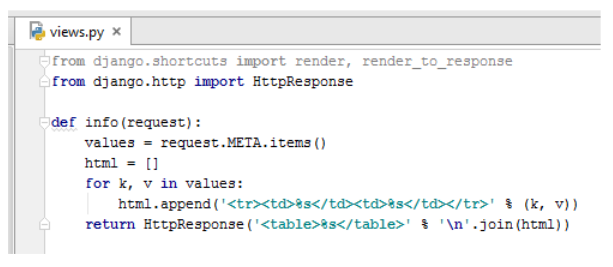
\includegraphics[scale=0.35]{12}
  \end{center}
\end{flushleft}

\subsubsection{Forms}

\begin{flushleft}
  Por excelência, os forms são os elementos HTML para enviar e receber dados
  do cliente para o servidor.

  Do lado do cliente (browser), o Form pode usar os métodos \textbf{GET} ou \textbf{POST} para
  enviar os dados que possui.

  Do lado do servidor, a view chamada pode usar os dicionários "\textbf{request.GET}" e "\textbf{request.POST}"
  para aceder aos dados recebidos.
\end{flushleft}

\begin{flushleft}
  \textbf{Exemplo:} Form para pesquisar livros por título

  \vspace{2mm}
  Definir o URL:

  \begin{center}
    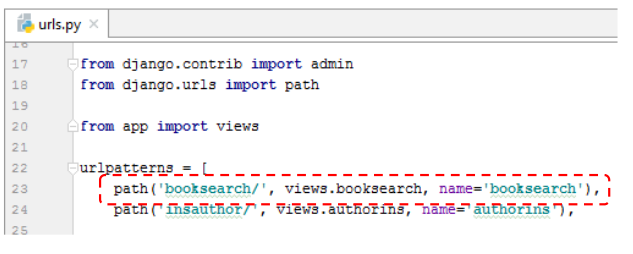
\includegraphics[scale=0.35]{13}
  \end{center}

  \pagebreak

  Definir a view:

  \begin{center}
    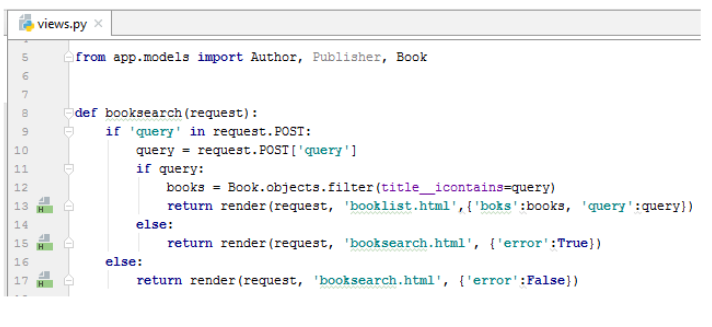
\includegraphics[scale=0.35]{14}
  \end{center}

  Definir o template para pesquisa:

  \begin{center}
    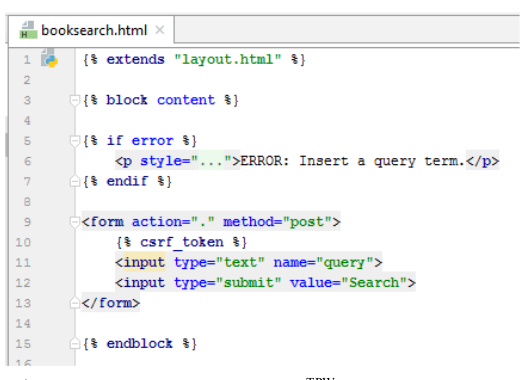
\includegraphics[scale=0.35]{15}
  \end{center}

  Definir o template para mostrar os resultados:

  \begin{center}
    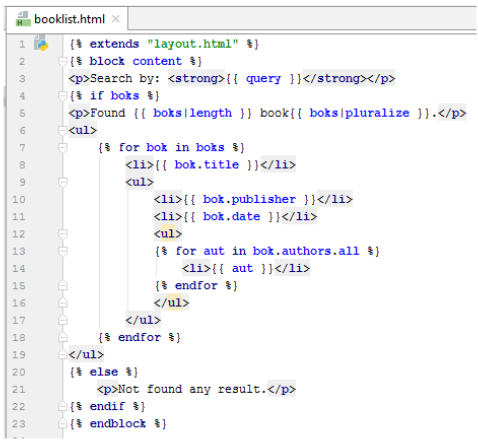
\includegraphics[scale=0.35]{16}
  \end{center}
\end{flushleft}

\pagebreak

\subsubsection{Classes Form e Django Forms}

\begin{flushleft}
  A classe \textbf{Form} descreve um formulário e determina como ele se comporta
  e como é apresentado no browser.

  Os campos da classe \textbf{Form} mapeiam para o formulário HTML como elementos
  \textbf{$<$input$>$}.
  \begin{itemize}
    \item Eles próprios são classes, que gerem os dados de um formulário
    e fazem a validação quando o formulário é submetido;
    \item São representados no browser como um "widget" HTML.
    Cada campo tem um default widget apropriado, mas estes podem ser
    overriden, se necessário;
  \end{itemize}
\end{flushleft}

\subsubsection{Instância de um Form}

\begin{flushleft}
  Numa instância de uma classe \textbf{Form}, podemos optar por
  deixar vazio ou pre-popular, por exemplo com:
  \begin{itemize}
    \item dados de uma instância de um modelo salvo (como é o caso do Django Admin para editar);
    \item dados que tenhamos coletado de outras fontes;
    \item dados recebidos de um submissão anterior de um formulário HTML;
  \end{itemize}

  O último caso é muito útil, pois permite os utilizadores reenviar informação
  sem terem que a reescrever.
\end{flushleft}

\subsubsection{Contruir um Form}

\begin{flushleft}
  Para contruir um formulário, normalmente escrevemos o código em HTML assim:

  \begin{center}
    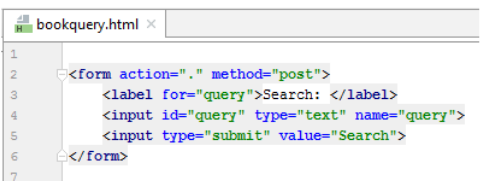
\includegraphics[scale=0.35]{17}
  \end{center}

  De facto, um formulário é bem mais complexo, incluindo vários campos, tipos de campos,
  restrições e regras de validação, pelo que seria bom ser mais fácil
\end{flushleft}

\subsubsection{Criando um Django Form}

\begin{flushleft}
  Para criar uma classe \textbf{Form} no Django, basta criar uma classe que herde de \textbf{forms.Form},
  no ficheiro "app/forms.py".

  \begin{center}
    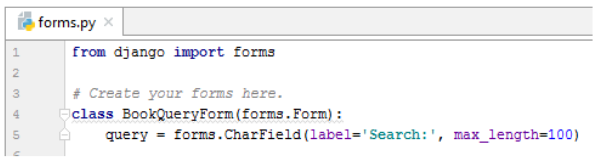
\includegraphics[scale=0.35]{18}
  \end{center}

  \pagebreak

  Depois criamos o template onde a class \textbf{Form} vai ser representada:

  \begin{center}
    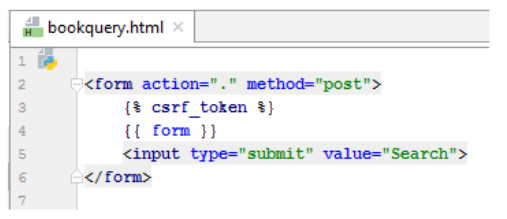
\includegraphics[scale=0.35]{19}
  \end{center}

  Quando renderizado, o formulário vai substituir o template tag \{\{ form \}\}
  com o label e o input definidos na classe \textbf{Form}.

  \vspace{2mm}

  A view será do tipo:

  \begin{center}
    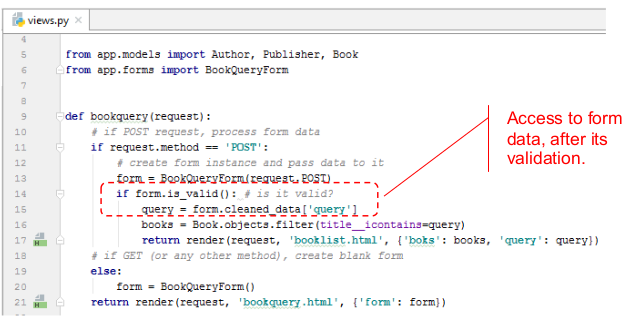
\includegraphics[scale=0.35]{20}
  \end{center}
\end{flushleft}

\subsubsection*{Os Campos}

\begin{flushleft}
  Os campos dos dados:
  \begin{itemize}
    \item Os dados submetidos com o formulário, usando \textbf{Form Fields}, podem
    ser validados usando a função \textbf{is\_valid()};
    \item Depois da validação, os dados podem ser acessados no dicionário
    \textbf{form.cleaned\_data};
    \item Os dados no dicionário já estão convertidos para tipos Python para
    uso imediato;
  \end{itemize}

  \vspace{2mm}

  \textbf{Exemplo} de Data Fields e a sua representação HTML:
  \begin{itemize}
    \item \textbf{BooleanField} - Checkbox Input;
    \item \textbf{CharField} - Text Input;
    \item \textbf{IntegerField} ou \textbf{FloatField} - Number Input;
    \item \textbf{DateField} e \textbf{TimeField} - Text Input;
    \item \textbf{ChoiceField} - Select;
    \item \textbf{MultipleChoiceField} - Select Mulriple;
    \item \textbf{FileField} - File Input;
  \end{itemize}

  Para já não é o mais aesthetically pleasing, mas corre direito e faz
  validação automática.

  \pagebreak

  É possível renderizar os Form Fields individualmente:

  \begin{center}
    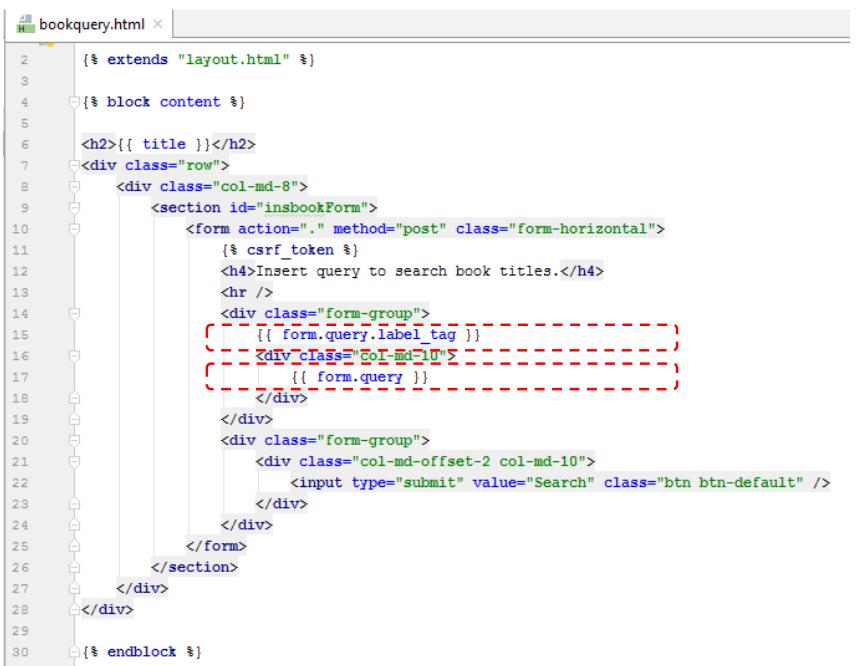
\includegraphics[scale=0.3]{21}
  \end{center}
\end{flushleft}

\subsection{Autentificação Django}

\begin{flushleft}
  O Django vem com um sistema de autentificação de utilizadores.
  Este sistema lida com contas de utilizadores, grupos, permissões e
  sessões de utilizadores.

  \vspace{2mm}

  Trata de ambos, a autentificação e a autorização.
  \begin{itemize}
    \item \textbf{Autentificação} - Verificar que o utilizador é quem diz ser;
    \item \textbf{Autorização} - Determina o que o utilizador autentificado tem permissão para fazer;
  \end{itemize}  

  Implementa:
  \begin{itemize}
    \item Utilizaddores, grupos e permissões;
    \item Ferramentas de Forms e view para "loggar" utilizadores ou restringir conteúdo;
    \item Hashing de passwords;
  \end{itemize}
\end{flushleft}

\subsubsection{Autentificação}

\begin{flushleft}
  Para usar o sistema de autentificação, temos de ver se os seguintes
  módulos estão incluídos:

  \begin{center}
    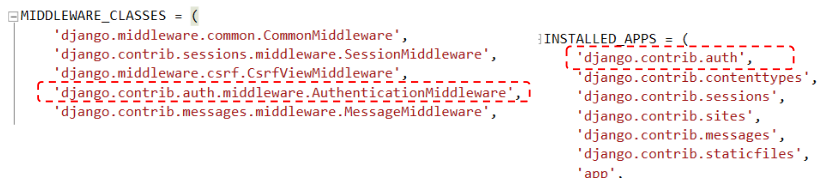
\includegraphics[scale=0.35]{22}
  \end{center}

  Além disso, a base de dados deve estar iniciada, senão: \textbf{python manage.py migrate}
\end{flushleft}

\pagebreak

\subsubsection{Criar Login e Logout}

\begin{flushleft}
  No ficheiro "app/urls.py" devemos adicionar as seguintes linhas:

  \begin{center}
    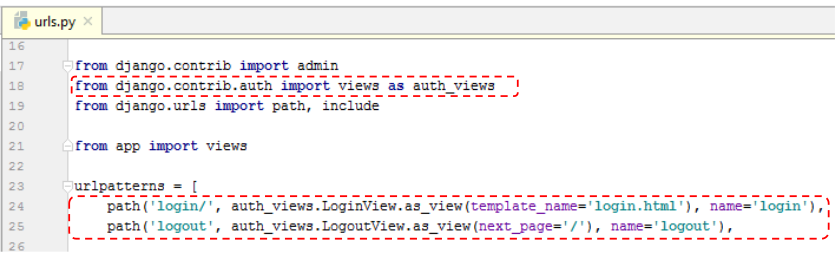
\includegraphics[scale=0.35]{23}
  \end{center}

  Usar o ficheiro "login.html" par criar o template do login, e fazer as seguintes alterações:

  \begin{center}
    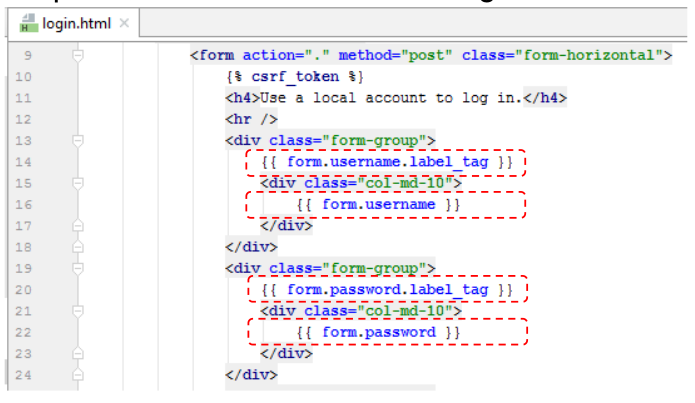
\includegraphics[scale=0.35]{24}
  \end{center}

  Usar o ficheiro "loginpartial.html" para criar a área se vai mostrar o status do login, 
  para tal modificamos o ficheiro "layout.html":

  \begin{center}
    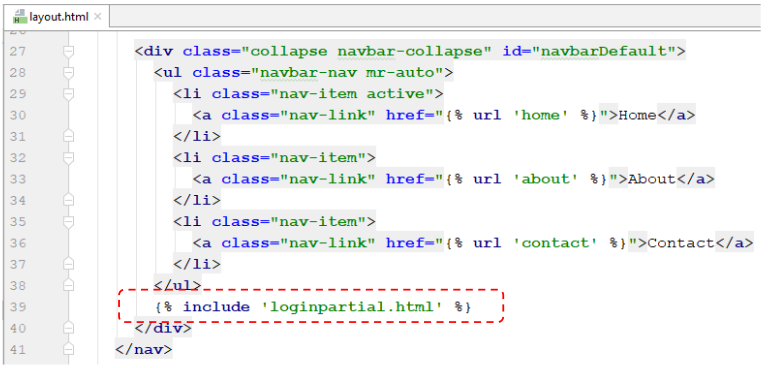
\includegraphics[scale=0.35]{25}
  \end{center}
\end{flushleft}

\pagebreak

\subsubsection{Autorização}

\begin{flushleft}
  A autorização pode ser gerida automaticamente pelo Django, através
  do objeto "\textbf{request.use}", é possível verificar se um dado
  utilizador está autentificado e se tem permissão para fazer operações.

  \begin{center}
    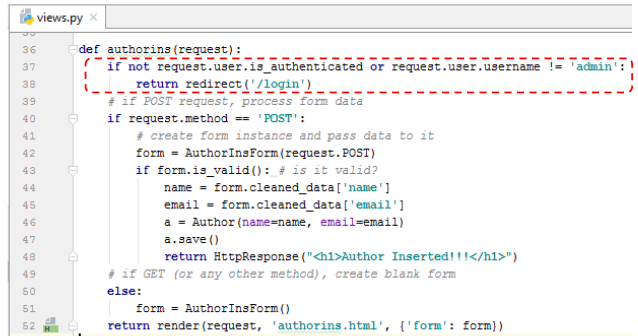
\includegraphics[scale=0.35]{26}
  \end{center}
\end{flushleft}

\subsection{Sessões Django}

\subsubsection{Estado}

\begin{flushleft}
  O protocolo HTTP é um protocolo sem estado (stateless), o que significa
  que não tem nenhum mecanismo para guardar o estado da conexão e, desta forma,
  não permite a criação de sessões.

  \vspace{2mm}

  Para tal, alguns mecanismos externos foram desenvolvidos em clientes web e
  servidores, que permitem guardar o dados do estado em várias conexões HTTP,
  produzindo sessões artificiais.

  \vspace{2mm}
  Mecanismos como:
  \begin{itemize}
    \item Cookies;
    \item Ferramentas de alto nível, usando BDs para gerir utilizadores,
    autentificações e sessões;
  \end{itemize}
\end{flushleft}

\subsubsection{Cookies}

\begin{flushleft}
  Uma cookie é uma peça de informação enviada pelo servidor web para o cliente,
  o browser, para ser guardada enquanto estão numa conexão.

  \vspace{2mm}

  É possível guardar algum tipo de informação nesta cookie, como o nome do
  utilizador por exemplo.

  \vspace{2mm}

  Este mecanismo de cookies é bastante usado por quase todos os web sites, mas
  possui algumas disvantagens:
  \begin{itemize}
    \item Salvar cookies no browser não é obrigatório, o que não permite
    oferecer garantia de um bom serviço;
    \item Cookies não podem ser usadas para guardar informação importante - não são seguras;
    \item Os servidores podem ser inibidos, em algum momento, de acessar informação crucial
    para continuar a interação com o cliente.
  \end{itemize}
\end{flushleft}

\pagebreak

\subsubsection{Sessões Django}

\begin{flushleft}
  O Django oferece um mecanismo de alto nível para o estabelecimento de sessões,
  o que permite salvar todo o tipo de informações no próprio seervidor. Esta informação
  é armazenada na base de dados.

  \vspace{2mm}

  Para usar este mecânismo, verifica se as seguintes linhas estão no ficheiro
  "\textbf{settings.py}".

  \begin{center}
    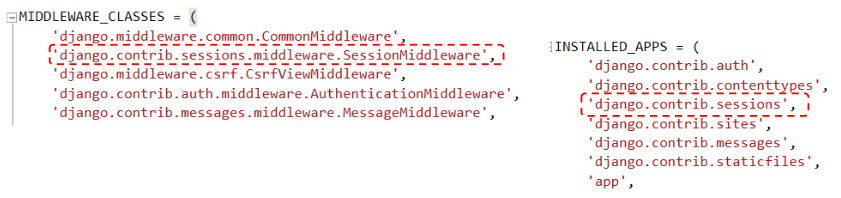
\includegraphics[scale=0.35]{27}
  \end{center}

  O Django gere automaticamente as sessões com os clientes de uma maneira
  simples e transparente. Utiliza o objeto "\textbf{request.session}" que
  é um dicionário.

  \begin{center}
    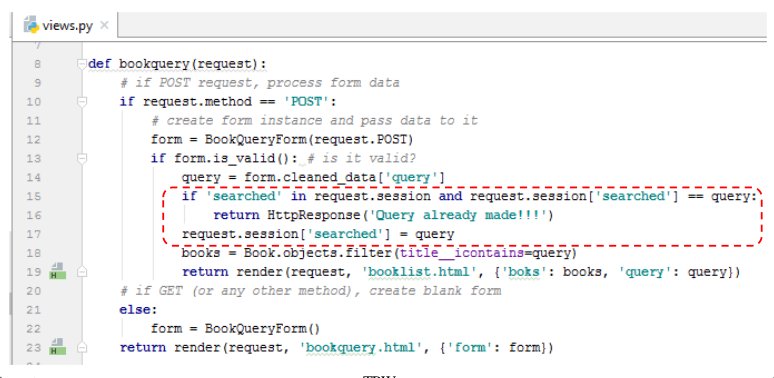
\includegraphics[scale=0.35]{28}
  \end{center}
\end{flushleft}

\pagebreak

\section{Produção - Deployment de Aplicações Web}

\subsection{Ambiente de Produção}

\begin{flushleft}
O ambiente de produção é o ambiente dado pelo computador servidor
onde a nossa aplicação web vai correr para consumo externo.

Isto inclui:
\begin{itemize}
  \item Hardware onde o website vai correr;
  \item Sistema Operativo (e.g Linux, Windows);
  \item Runtime das linguagens de programação e frameworks por cima das quais o website é escrito;
  \item O servidor web usado para servir páginas e outros conteúdos (e.g Apache, Nginx);
  \item O servidor da aplicação que passa pedidos "dinâmicos" entre a aplicação web e o servidor web;
  \item Bases de Dados das quais a nossa aplicação depende;
\end{itemize}

\vspace{2mm}

O computador servidor pode estar localizado fisicamente na nossa empresa e
conectado à Internet por um link rápido.

\vspace{1mm}

\textbf{OU}

\vspace{1mm}

Usar um computador servidor que está hosted "na cloud".
\begin{itemize}
  \item Neste caso, o nosso código corre num computador remota, ou possivelmente
  um computador "virtual", que é gerido por uma empresa de hosting (data center);
  \item O servidor remoto normalmente oferece algumu nível garantido de recursos
  de computação (e.g CPU, RAM, memória de disco, /dots) e conectividade à Internet
  por um preço fixo;
\end{itemize}

\end{flushleft}

\subsection{Ambiente de Produção - IaaS}

\begin{flushleft}
  \textbf{IaaS} - Infrastructure as a Service - é um hardware de computação/networking
  acessado remotamente, fornecido por um serviço de hosting.

  \vspace{2mm}

  Muitos fornecedores de IaaS oferecem opções para pre-instalar um dado Sistema Operativo,
  no qual devemos instalar componentes do ambiente de produção.

  \vspace{2mm}

  Outros vendedores permitem selecionar um ambiente pré-configurado, que inclui
  uma dada web framework, e.g Django, e um web-server setup.
\end{flushleft}

\pagebreak

\subsection{Ambiente de Produção - PaaS}

\begin{flushleft}
  \textbf{PaaS} - Platform as a Service - é outro tipo de serviço de hosting onde
  a plataforma de hosting trata:
  \begin{itemize}
    \item de grande parte do ambiente de produção - servidor web, servidor de aplicação,
    load balancers;
    \item e da maior parte que precisamos para escalar a nossa aplicação web;
  \end{itemize}

  PaaS torna o deployment bastante fácil, uma vez que só precisamos de nos concentrar
  na nossa aplicação web e não em toda a outra infrastrutura do servidor.
\end{flushleft}

\subsection{Escolher um Serviço de Hosting}

\begin{flushleft}
  Problemas a ter em conta:
  \begin{itemize}
    \item O quão provável é o nosso website estar ocupado e o custo dos dados e
    os recursos de computação necessários para suportar o tráfego;
    \item O nível de suporte para escalar horizontalmente (adicionar mais máquinas)
    e verticalmente (upgrade para m´quinas mais poderosas) e os custos de o fazer;
    \item Onde o fornecedor tem data centers, e por isso, onde o acesso é mais provável de ser mais rápido;
    \item O histórico do uptime do fornecedor e a performance do downtime;
    \item Ferramentas dadas para gerir o site, se são fáceis de usar e se são seguras (e.g SFTP vs FTP);
    \item Inbuilt Frameworks para monitorizar o servidor;
    \item Saber os limites. Alguns hosts bloquiam delibradamente certos serviços (e.g email).
    Outros oferece, um certo número de horas de "live time" em alguns pacotes de preços, ou apenas
    fornecem uma pequena quantidade de memória;
    \item Benefícios adicionais. Alguns fornecedores oferecem domain names e suporte para certificados SSL
    que teriamos, caso contrário, de comprar.
    \item Se o tier "grátis" que estamos a usar expira ao longo do tempo e se o custo de migração
    para um tier mais caro significa que seria melhor ter usado outro serviço de hosting desde o início;
  \end{itemize}
\end{flushleft}

\end{document}